\let\negmedspace\undefined
\let\negthickspace\undefined
\documentclass[journal]{IEEEtran}
\usepackage[a5paper, margin=10mm, onecolumn]{geometry}
%\usepackage{lmodern} % Ensure lmodern is loaded for pdflatex
\usepackage{tfrupee} % Include tfrupee package

\setlength{\headheight}{1cm} % Set the height of the header box
\setlength{\headsep}{0mm}     % Set the distance between the header box and the top of the text

\usepackage{gvv-book}
\usepackage{gvv}
\usepackage{cite}
\usepackage{amsmath,amssymb,amsfonts,amsthm}
\usepackage{algorithmic}
\usepackage{graphicx}
\usepackage{textcomp}
\usepackage{xcolor}
\usepackage{txfonts}
\usepackage{listings}
\usepackage{enumitem}
\usepackage{mathtools}
\usepackage{gensymb}
\usepackage{comment}
\usepackage[breaklinks=true]{hyperref}
\usepackage{tkz-euclide} 
\usepackage{listings}
% \usepackage{gvv}                                        
\def\inputGnumericTable{}                                 
\usepackage[latin1]{inputenc}                                
\usepackage{color}                                            
\usepackage{array}                                            
\usepackage{longtable}                                       
\usepackage{calc}                                             
\usepackage{multirow}                                         
\usepackage{hhline}                                           
\usepackage{ifthen}                                           
\usepackage{lscape}
\usepackage{circuitikz}
\tikzstyle{block} = [rectangle, draw, fill=blue!20, 
    text width=4em, text centered, rounded corners, minimum height=3em]
\tikzstyle{sum} = [draw, fill=blue!10, circle, minimum size=1cm, node distance=1.5cm]
\tikzstyle{input} = [coordinate]
\tikzstyle{output} = [coordinate]
\begin{document}



\textbf{Question:} 
Find the values of $k$ for which the points $A(k+1, 2k)$, $B(3k, 2k+3)$, $C(5k-1, 5k)$ are collinear. 
\vspace{0.5cm}

\textbf{Solution:}

First, form the difference vectors:
\[
 B - A = 
\begin{pmatrix}
3k - (k+1) \\ (2k+3) - 2k
\end{pmatrix}
=
\begin{pmatrix}
2k - 1 \\ 3
\end{pmatrix}
\]
\[
  C - A =
\begin{pmatrix}
(5k-1) - (k+1) \\ 5k - 2k
\end{pmatrix}
=
\begin{pmatrix}
4k - 2 \\ 3k
\end{pmatrix}
\]

Form the matrix:
\[
M = \begin{pmatrix}
2k-1 & 3 \\
4k-2 & 3k
\end{pmatrix}
\]

For the points to be collinear, the rank of $M$ must be $1$. Perform the row operation:
\[
R_2 \to -\frac{4k-2}{2k-1}R_1 + R_2 \qquad \text{(for $2k-1 \neq 0$)}
\]

Which gives:
\[
\begin{pmatrix}
2k-1 & 3 \\
0 & 3k - \frac{3(4k-2)}{2k-1}
\end{pmatrix}
\]

Set the second row entry to zero for rank $1$:
\[
3k - \frac{3(4k-2)}{2k-1} = 0
\]
\[
3k = \frac{3(4k-2)}{2k-1}
\]
\[
3k(2k-1) = 3(4k-2)
\]
\[
6k^2 - 3k = 12k - 6
\]
\[
6k^2 - 15k + 6 = 0
\]
\[
2k^2 - 5k + 2 = 0
\]

Solving for $k$:
\[
k = \frac{5 \pm 3}{4}
\]
\[
k = 2 \quad \text{or} \quad k = \frac{1}{2}
\]
\begin{figure}
    \centering
    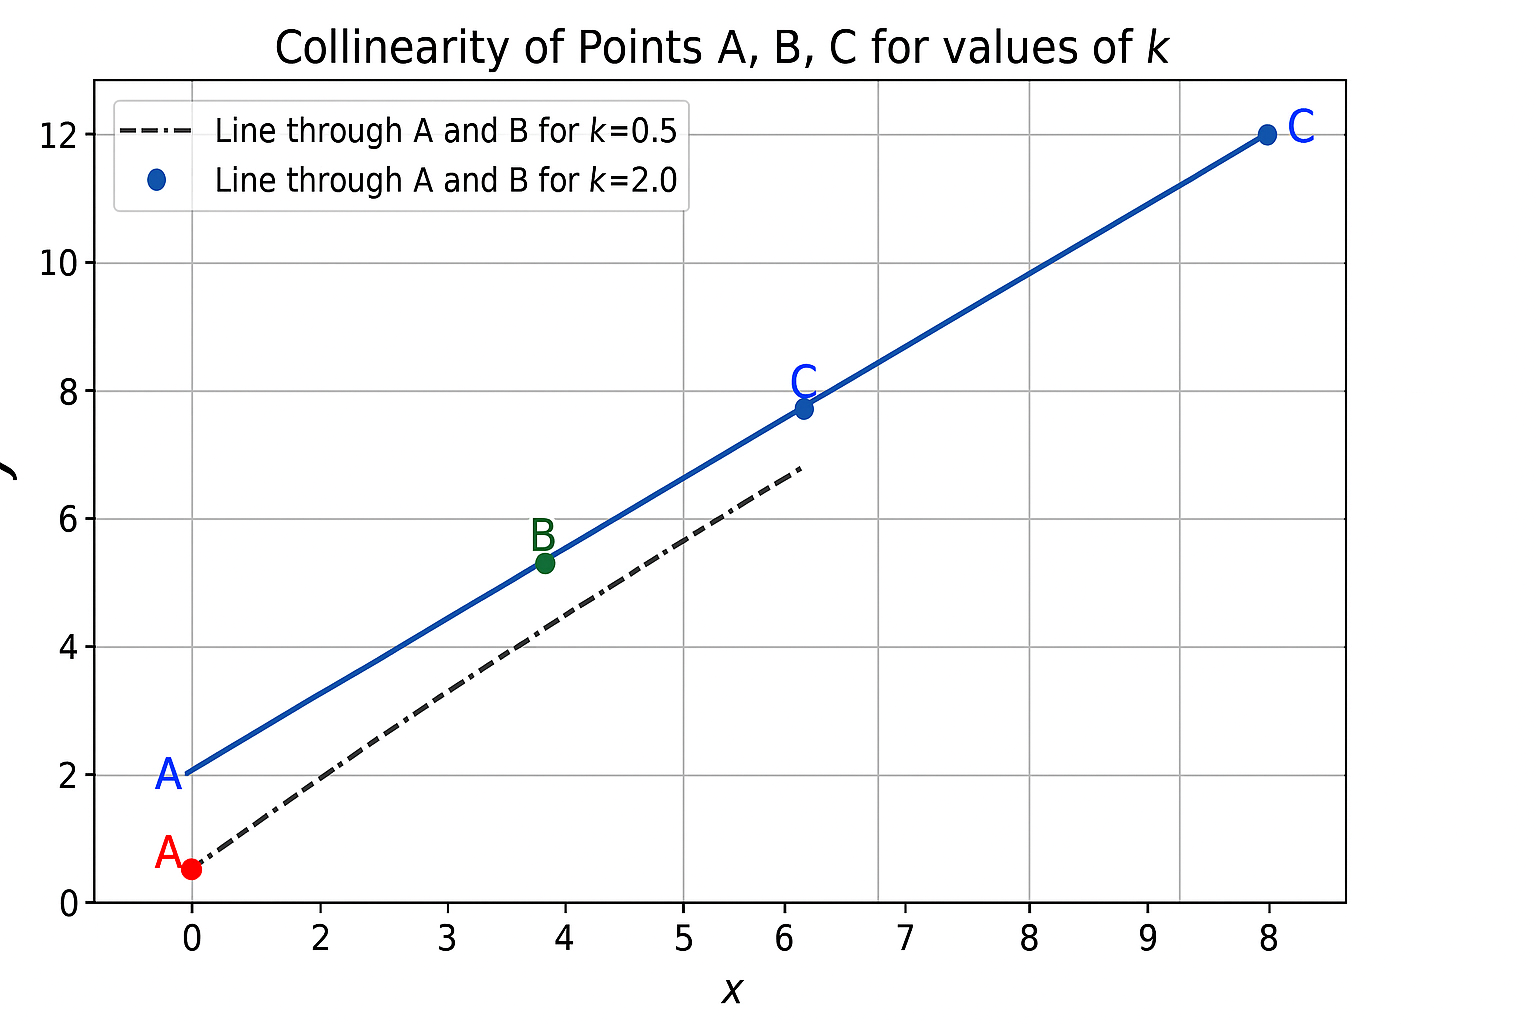
\includegraphics[width=1\linewidth]{figs/plot.png}
    \caption{plot}
    \label{fig:placeholder}
\end{figure}

\end{document}
